\documentclass[tikz,border=5pt]{standalone}
\usepackage{fontspec}
\setmainfont{Times New Roman}
\usepackage{unicode-math}
\setmathfont{Cambria Math}
\usetikzlibrary{shapes.geometric,positioning,fit,backgrounds,arrows.meta,calc,matrix}

\begin{document}
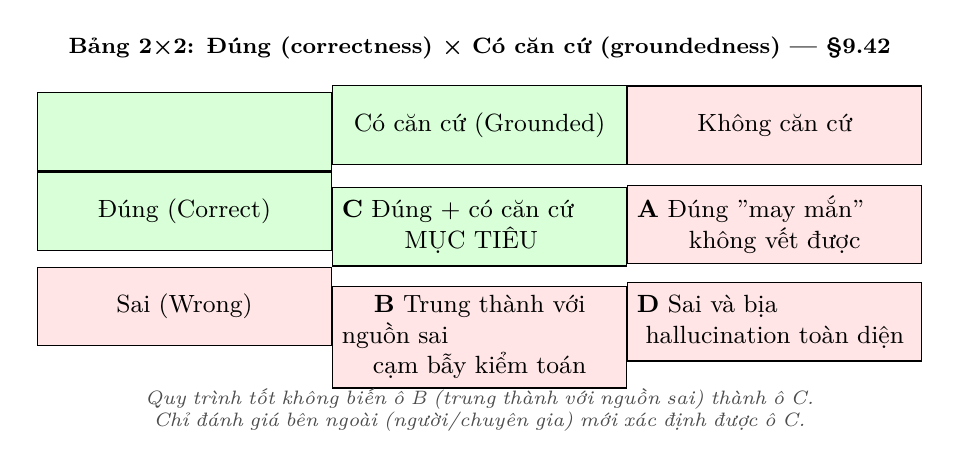
\begin{tikzpicture}
\node[font=\footnotesize\bfseries, align=center] at (0, 2.4) {Bảng 2×2: Đúng (correctness) × Có căn cứ (groundedness) — §9.42};

\matrix (m) [matrix of nodes, nodes={rectangle, draw, align=center, text width=3.5cm, minimum height=1.0cm, font=\small}, column sep=0pt, row sep=0pt] {
  |[fill=green!15]| & |[fill=green!15]| Có căn cứ (Grounded) & |[fill=red!10]| Không căn cứ \\
  |[fill=green!15]| Đúng (Correct) & |[fill=green!15]| \textbf{C} Đúng + có căn cứ \newline ~~~MỤC TIÊU~~~ & |[fill=red!10]| \textbf{A} Đúng "may mắn" \newline không vết được \\
  |[fill=red!10]| Sai (Wrong) & |[fill=red!10]| \textbf{B} Trung thành với nguồn sai \newline cạm bẫy kiểm toán & |[fill=red!10]| \textbf{D} Sai và bịa \newline hallucination toàn diện \\
};

\node[font=\scriptsize\itshape, text=gray!60!black, align=center, text width=9cm] at (0, -2.2)
  {Quy trình tốt không biến ô B (trung thành với nguồn sai) thành ô C.\\Chỉ đánh giá bên ngoài (người/chuyên gia) mới xác định được ô C.};

\end{tikzpicture}
\end{document}